\chapter{Data Sample and Event Selection}\label{section:star_data_sample}\label{section:star_trigger_selection}
The data sample used in this analysis was collected in proton-proton collisions at centre-of-mass energy of $\sqrt{s}=200$~GeV during RHIC Run 15. %Data from the RP related triggers is stored in a~special data stream.

\begin{figure}[b!]
	\centering
	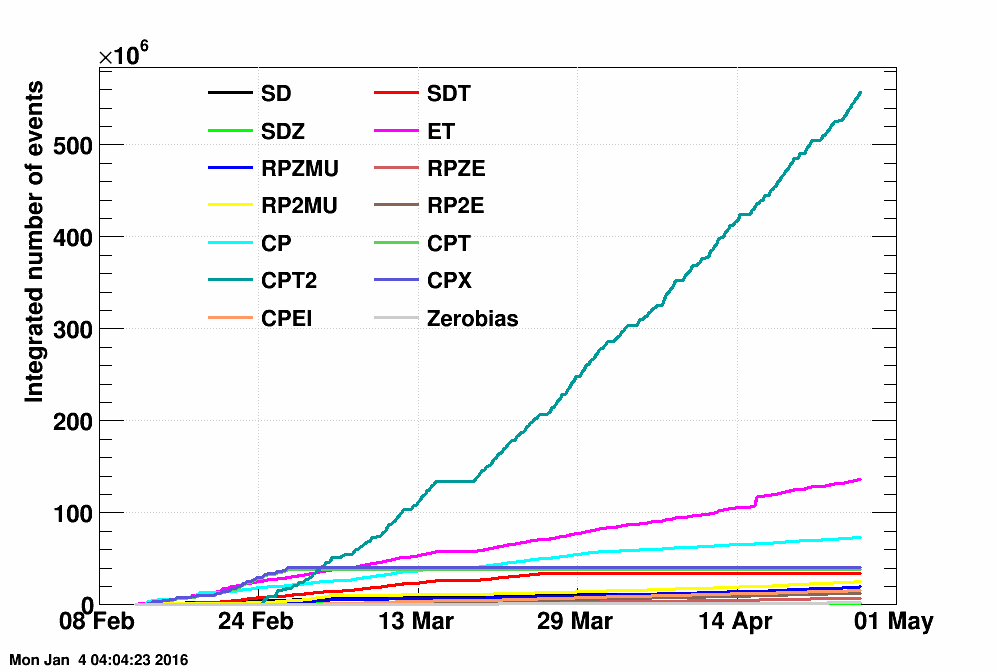
\includegraphics[width=.6\textwidth]{chapters/dataSampleSTAR/img/nEvents.png}
	\caption{Cumulative number of events collected for each trigger in the~\ac{RP} data stream during Run 15~\cite{pp2ppTrigers,runLogBrowser}. }
	\label{fig:lumiRHIC}
\end{figure}

All of the studies in this analysis use data from only the SDT trigger condition, which was the main trigger designed for SD studies in Run 15. The~logic of the~trigger  was formed by the following conditions combined with the logical AND:
\begin{enumerate}
	\item RP\_EOR $||$ RP\_WOR - signal in at least one RP on any side of the STAR central detector,
	\item veto on any signal in small BBC tiles or ZDC on the triggered RP  side of the~STAR central detector,
	\item at least two TOF hits.
\end{enumerate}
The~above  requirements were imposed in accordance with the diffractive event topology. Veto on any signal in small BBC tiles and ZDC allowed to accept only events with rapidity gap and reject diffractive events with simultaneous pile-up event. The requirement of at least two TOF hits was applied to ensure activity in the mid-rapidity.


Integrated luminosity delivered by the RHIC to the STAR experiment in $pp$ collisions during Run 15 amounts to $185.1$~pb$^{-1}$~\cite{RHIC:rhicRunLuminosity}, whereas about $34.4$M SDT events were gathered by the STAR detector, shown in Fig.~\ref{fig:lumiRHIC}, which corresponds to $16$~nb$^{-1}$ of integrated luminosity.
%\FloatBarrier
